% _example: this file is yours. Edit the caption, the label, the
% placement ([t], [h!], ...), or wrap it in a starred figure* for a wide one.
% plotplate never overwrites it; it rewrites the panels in the file included below.
\begin{figure}[tbp]
  \centering
  % Generated by plotplate from layout.yaml (_example). Do not edit by hand.
% Requires \usepackage{graphicx}. Panels are included at natural size (scale 1.0).
\providecommand{\plotplatePanelLabel}[1]{{\fontsize{8pt}{8pt}\selectfont\sffamily\bfseries #1}}%
{\setlength{\unitlength}{1mm}%
\begin{picture}(183.00,100.00)%
\put(0.00,52.00){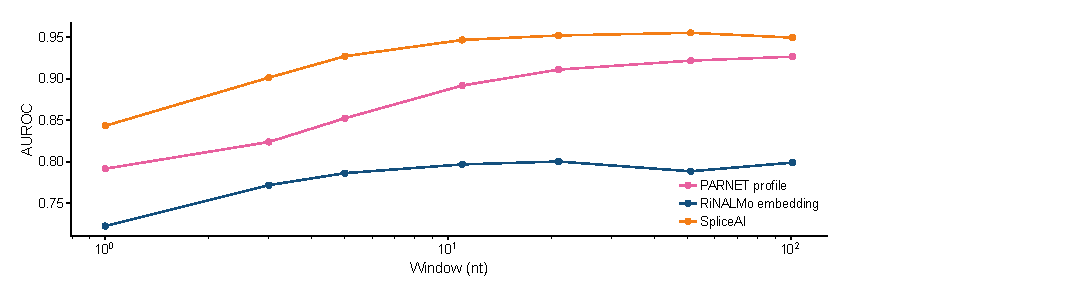
\includegraphics{panels/A.pdf}}% panel A
\put(0.00,0.00){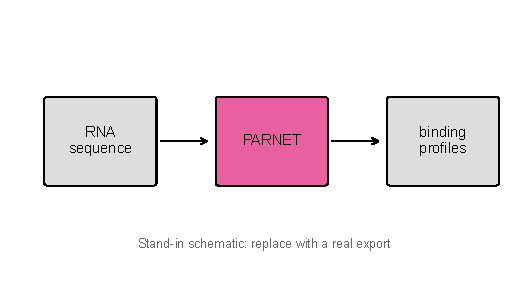
\includegraphics{panels/B.pdf}}% panel B
\put(93.50,0.00){
\includegraphics{panels/C.pdf}}% panel C
\put(0.00,100.00){\makebox(0,0)[lt]{\plotplatePanelLabel{a}}}%
\put(0.00,48.00){\makebox(0,0)[lt]{\plotplatePanelLabel{b}}}%
\put(93.50,48.00){\makebox(0,0)[lt]{\plotplatePanelLabel{c}}}%
\end{picture}}%
%
  \caption{...}
  \label{fig:_example}
  % To reference one panel (\ref{fig:_examplea} prints 7a), load subcaption in the
  % preamble and uncomment the lines below. They print nothing and take no space.
  % \begin{subfigure}[t]{0pt}\phantomsubcaption\label{fig:_examplea}\end{subfigure}%  panel A
  % \begin{subfigure}[t]{0pt}\phantomsubcaption\label{fig:_exampleb}\end{subfigure}%  panel B
  % \begin{subfigure}[t]{0pt}\phantomsubcaption\label{fig:_examplec}\end{subfigure}%  panel C
\end{figure}
